\section{User Manual}
  
  \renewcommand\imagewidth{0.4\textwidth}
  
  In this appendix the main user actions are shown and the process to execute them is detailed.
 
  \subsection {Software Requirements}
  
    In order to successfully run the application the user needs an updated version of Google Chrome\footnote{At the time of this writing the latest Google Chrome version is 52.0.2743.116 and the latest Google Chrome Canary version is 54.0.2829.0.} with the flags \textit{\#enable-webgl-draft-extensions} and \textit{\#enable-unsafe-es3-apis} active so that WebGL 2.0 is available.
      
  \subsection {Loading a Base Surface}
  
    There are two options to load a base surface. The first option is to simply open a PNG image that contains a height map of the surface which will be set as the current base surface. The second option is to open a previously exported result ZIP file (see section \ref{app:sec:saving}) that will set the base surface used to generate that result as the current base surface and will add that result to the history panel. Both this actions are accessible from the File menu in the application's Top Bar as shown in Figure \ref{fig:topbar-filemenu}.
  
    \begin{figure}[H]
      \centering
      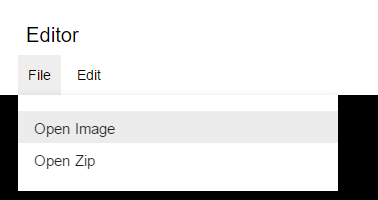
\includegraphics[width=\imagewidth]{images/screenshots/TopBar-FileMenu}
      \caption{Top Bar - File Menu}
      \label{fig:topbar-filemenu}
    \end{figure}
  
  \newpage
  
  \subsection {Adding Details}
  
    After loading the base surface the option to add details becomes available in the Edit menu of the application's Top Bar, as shown in Figure \ref{fig:topbar-editmenu}. 
  
    \begin{figure}[H]
      \centering
      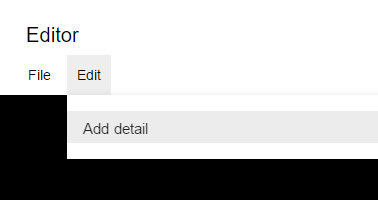
\includegraphics[width=\imagewidth]{images/screenshots/TopBar-EditMenu}
      \caption{Top Bar - Edit Menu}
      \label{fig:topbar-editmenu}
    \end{figure}
    
    When the user clicks on the "Add detail" option, a panel will appear on the left with the available parameters (see Table \ref{table:parameters} for the available parameters). This panel is divided in two parts: the generation phase, shown in Figure \ref{fig:leftbar-generation}, and the blend phase, presented in Figure \ref{fig:leftbar-blendphase}.
    
    \begin{figure}[H]
      \centering
      \vcenteredhbox{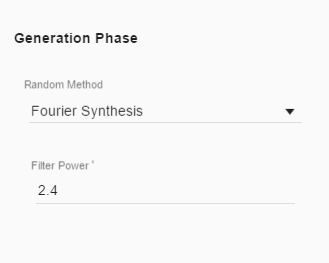
\includegraphics[width=\imagewidth]{images/screenshots/LeftBar-Generation-Fourier}}
      \vcenteredhbox{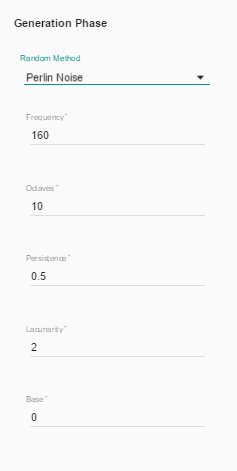
\includegraphics[width=\imagewidth]{images/screenshots/LeftBar-Generation-Noise}}
      \caption{Left Panel - Generation Phase}
      \label{fig:leftbar-generation}
    \end{figure}
    
    The parameters visible in the generation phase will depend on the random generation method. In Figure \ref{fig:leftbar-generation} the left image shows the Fourier Filtering method and the right image shows the Noise Synthesis method, as the parameters are the same for both Perlin and Simplex noise.
  
    \begin{figure}[H]
      \centering
      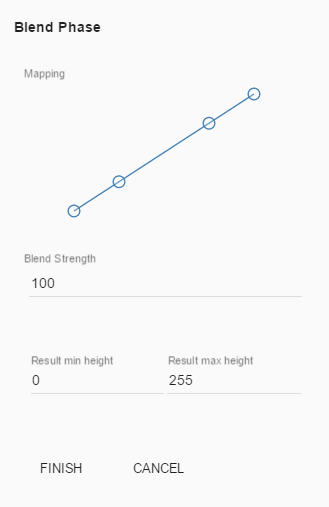
\includegraphics[width=\imagewidth]{images/screenshots/LeftBar-BlendPhase}
      \caption{Left Panel - Blend Phase}
      \label{fig:leftbar-blendphase}
    \end{figure}
   
    
    In the blend phase the user can change the spline mapping control points by simply clicking and dragging them. While the middle ones can be dragged both vertically and horizontally, the first and the last one can only be dragged vertically in order to keep the spline bounds fixed. Additionally the control points order cannot be changed either.
    
    All the controls shown in this section will trigger an automatic update to the terrain preview. When the user is satisfied with the terrain he can submit the result to the right panel by clicking the "Finish" button or, if he wishes to undo the parameter changes he can do so by pressing the "Cancel" button, both of which are placed in the bottom of the Left panel.
  
  \subsection {Saving the Results} \label{app:sec:saving}
  
    After submitting the terrain, the result is added to the Right panel (Figure \ref{fig:rightbar}), also known as the History. Here the user can see the parameters that were used in the enhancement process, as well as, export a certain result to a file. In the right side of the panel a screenshot of each of the history entries is displayed which, when clicked, will change the contents of the left side of the panel to the parameters used to generate the selected terrain. 
    
    \begin{figure}[H]
    	\centering
    	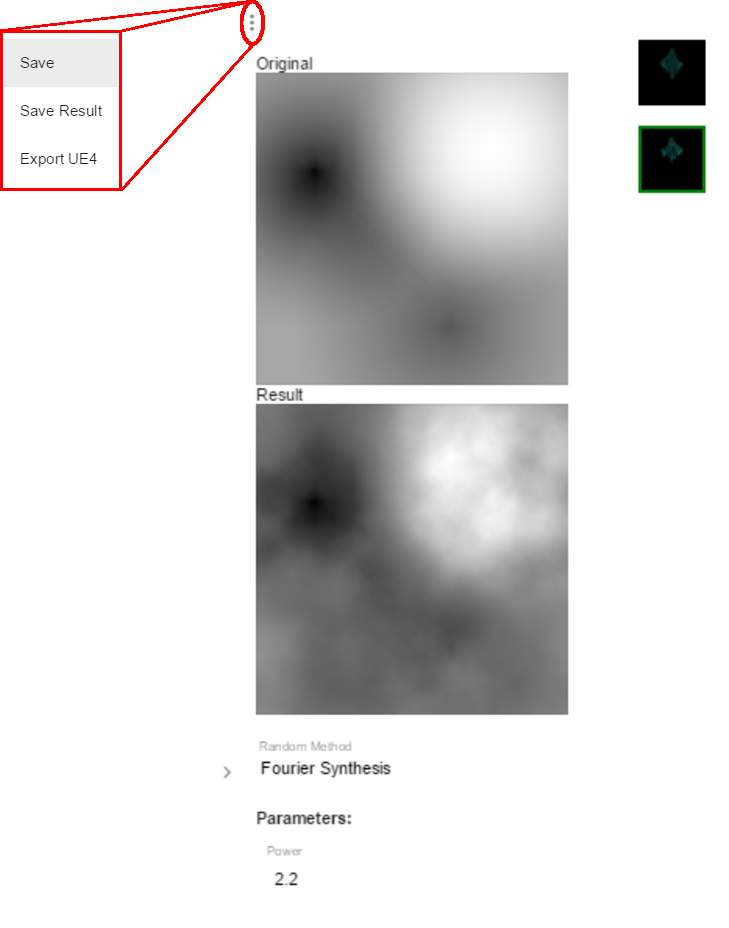
\includegraphics[width=0.75\textwidth]{images/screenshots/RightBar-WithMenu-1}
    	\caption{Right Panel}
    	\label{fig:rightbar}
    \end{figure}
    
    Additionally the user can also export the result to the formats referred in Section \ref{sec:io_formats} by clicking on the three dotted button on the top left corner of the panel and selecting the desired format.
  
    
  
  
  
  
